\chapter{État de l'art des attaques sur SSL/TLS}

\begin{figure}[H]
  \caption{Historique des attaques SSL/TLS (source : Cloudflare \cite{cloudflare})}
  \fbox{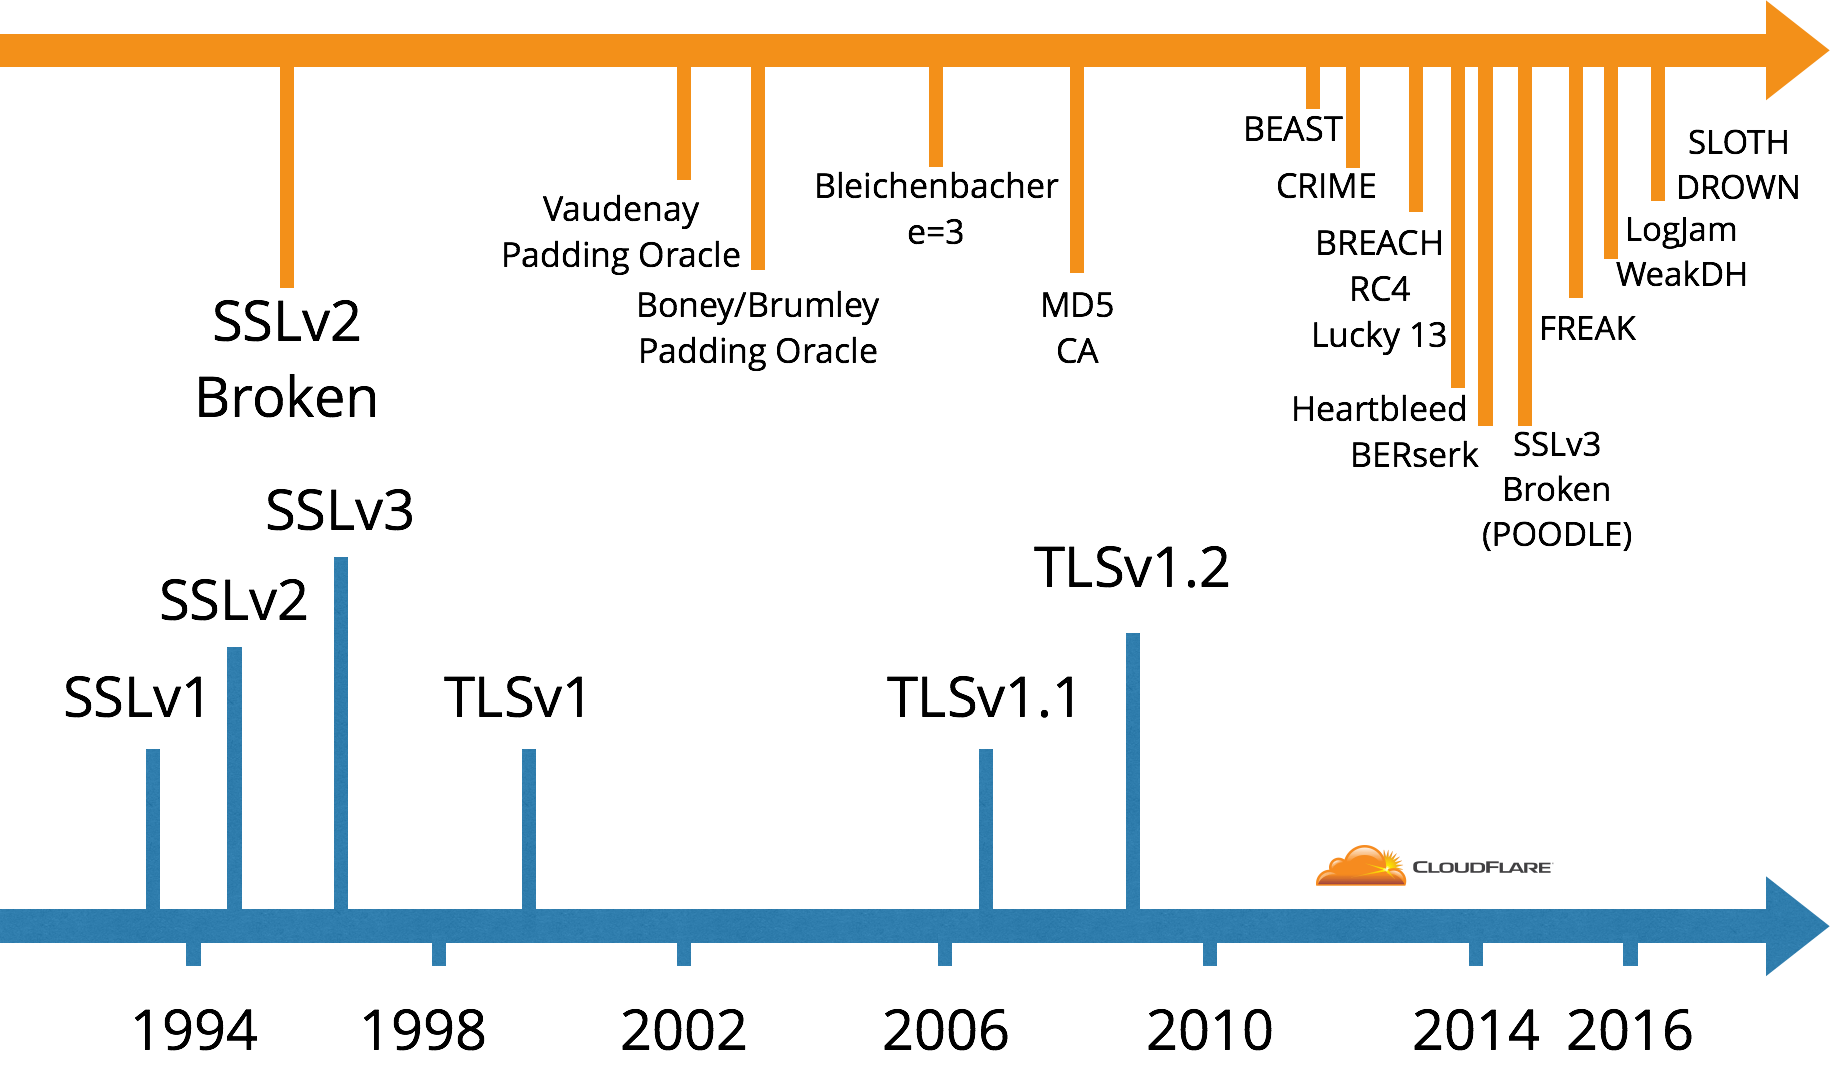
\includegraphics[width=\textwidth]{./history-tls-attacks.png}}
\end{figure}

\section{Attaques liées à l'implémentation}

\subsection{Heartbleed (2014)}
Cette faille est une faille d'OpenSSL basée sur SSL/TLS. Cette vulnérabilité permet de lire la mémoire du serveur. Cette faille est due à une erreur de programmation dans la focntion Heartbeat qui permet de maintenir la connexion sécurisée entre le navigateur et le serveur.

En effet, l'attaquant peut mentir sur le poids de la requête qu'il envoit et obtenir des données qui ne lui était pas destinées mais qui se trouve en mémoire. Il peut donc récupérer les informations comme des identifiants, des mots de passes, des cookies de sessions ou encore des clés de chiffrements \cite{heartbleed}.

\subsection{BERserk (2014)}
Cette faille concerne la bibliothèque Network Security Services présente dans certains navigateurs. L'attaque repose sur la falsification de signature numérique. La faille est présente à cause de l'analyse incorrecte de messages codés en ASN.1 lors de la vérification de signatures RSA. Les messages ASN.1 sont constitués de diverses parties codées à l'aide de BER (Basic Encoding Rule) et DER (Distinguished Encoding Rules). C'est une variation de la faille Bleichenbacher PKCS\#1. Cette attaque exploite le fait que la longueur d'un champ dans le codage BER peut être utilisée pour utiliser de nombreux octets de données. Dans les implémentations vulnérables, ces octets sont ensuite ignorés lors de l'analyse\cite{berserk}.

\section{Attaques liées à la cryptographie}

\subsection{BEAST (2011)}
L'attaque BEAST, Browser Exploit Against SSL/TLS concerne SSL 3.0 et TLS 1.0. L'attaquant, placé en Man-in-the-Middle, peut déchiffrer les données échangées entre le serveur et le client grâce à une vulnérabilité d'implémentation du mode CBC, Cipher Block Chaining. L'attaque se fait côté client en injectant des paquets dans le flux TLS. Cette technique est qualifiée d'attaque à clair connu. La faille du protocole réside dans le chiffrement par bloc. En effet, les blocs sont chiffrés les uns après les autres en utilisant le précédent \cite{beast}.

Voici le déroulement de l'attaque :

\begin{enumerate}
\item Injection du code chez la victime
\item La victime envoie de données forgées via SSL
\item L'attaquant écoute le trafic
\item Il renvoit les informations nécessaires à son code injecté
\item La victime réenvoit les données forgées et on repète les deux étapes précédentes
  \item L'attaquant dérive tous les cookies
\end{enumerate}

\subsection{Cassage de RC4 (2013)}

Blablabla \cite{rc4}

\subsection{Lucky13 (2013)}

Blablabla \cite{lucky13}

\subsection{Logjam (2015)}

Blablabla \cite{logjam}

\subsection{DROWN (2016)}

Blablabla \cite{drown}

\subsection{SLOTH (2016)}

Blablabla \cite{sloth}

\subsection{SWEET32 (2016)}

Blablabla \cite{sweet32}

\subsection{ROBOT (2017)}

Blablabla \cite{robot}

\section{Attaques sur le protocole}

\subsection{CRIME (2012)}

CRIME (compression ratio info-leak made easy), utilise une faille de l'algorithme de compression utilisé par TLS. Cette attaque vise surtout les cookies de sessions. L'idée est d'envoyer des caractères aléatoires dans un cookie forgé et de comparer la compression de ce dernier avec le cookie originel du client. Si le cookie forgé est partiellement compressé, on peut inférer qu'une partie de ce dernier correspondant au cookie du client. On procède ainsi par étapes successives pour retrouver le cookie et voler la session de la victime.

Cette attaque nécessite que l'attaquant se place en MITM pour pouvoir observer la taille du chiffré envoyé par le client mais également pouvoir envoyer des requêtes forgées par l'attaquant lui-même \cite{crime}.

\subsection{BREACH (2012)}

L'attaque BREACH (browser reconnaissance and exfiltration via adaptive compression of hypertext) est en grande partie similaire à CRIME vue plus haut. Cette fois ci ce n'est pas la compression TLS mais plutôt celle effectuée par HTTP qui est visée \cite{breach}.

\subsection{POODLE (2014)}

L'anagramme POODLE signifie "padding oracle on downgraded legacy encryption". L'attaque concerne surtout les chiffrements SSL 3.0, bien qu'une variante de la faille fut trouver sur TLS un peu après.
Le padding dont parle le nom de l'attaque vient des méthodes de chiffrements cryptographiques. Lorsqu'un message envoyé un trop court pour l'algorithme de chiffrement, on lui rajoute une partie arbitraire, le "padding" pour qu'on puisse appliquer l'algorithme dessus.

Bien que le TLS soit un protocol plus sûr que SSL et recommandé aujourd'hui, de nombreux serveurs continuent d'accepter le SSL 3.0 si une connexion par TLS venait à être impossible. L'attaque POODLE se sert de ce fait pour forcer la connexion à se faire en SSL.

La vulnérabilité en elle-même vient de la façon dont sont encodés les blocs de donnés avec SSL. L'attaquant a besoin de deux choses pour se faire :

\begin{enumerate}
    \item L'attaquant doit pouvoir changer une partie du message injecté par le client dans l'algorithme
    \item Il doit avoir un retour sur le texte chiffré par SSL.
\end{enumerate}

Ces deux conditions peuvent s'exécuter avec par exemple une attaque en homme du milieu. L'attaquant doit toutefois avoir un contrôle également sur le client pour modifier le padding, ce qui est une tâche supplémentaire à effectuer.

En modifiant le padding, l'attaque permet de récupérer un byte d'information du message initial en envoyant un maximum de 256 requêtes. Cela peut ammener l'attaquant à envoyer énormément de réquêtes pour obtenir le message dans son intégralité.

L'avantage de cette attaque est qu'elle ne nécessite pas de connaître la clef utilisée pour le chiffrement \cite{poodle}.

\subsection{FREAK (2015)}

FREAK (factorising RSA export keys) a pour origine l'exportation de la cryptographie des USA qui gardait pour eux les meilleurs systèmes et partageait les moins bons avec le reste du monde, afin que la NSA puisse les craquer avec leur puissance de calcul supérieur.

Vers 2010 avec la montée en puissance constante des ordinateurs, tout le monde est maintenant capable avec un "bon pc" de craquer ces clés plus faibles, les "export-keys".

Le but de l'attaque est donc de forcer la connexion client/serveur de la victime a utiliser ces clefs plus faibles au lieu des clefs RSA standards plus fortes utilisées aujourd'hui \cite{freak}.

\subsection{WeakDH (2015)}

Blablabla \cite{weakdh}

\section{Attaques de l'homme du milieu}

\subsection{SSLsniff (2002)}

Blablabla \cite{sslsniff-website}

\subsection{SSLstrip (2009)}

Blablabla \cite{sslstrip-website}

\subsection{HTTPS interception}

Blablabla \cite{https-interception}
